\documentclass[12pt]{article}

\usepackage[T2A]{fontenc}
\usepackage[utf8]{inputenc}
\usepackage[english, russian]{babel}

\usepackage[letterpaper,top=2cm,bottom=2cm,left=1.5cm,right=1.5cm,marginparwidth=1.75cm]{geometry}
\usepackage{float}
%\usepackage[stable]{footmisc}

\usepackage{amsmath,amssymb}
\usepackage{graphicx}
\usepackage[colorlinks=true, allcolors=blue]{hyperref}
\hypersetup{unicode=true}
\usepackage{url}
\usepackage{longtable,booktabs,array}
\usepackage{tablefootnote}
\usepackage{circuitikz}
\usetikzlibrary{fit}
\usepackage{multicol}
\usepackage{soul}
\usepackage{listings}

\title{Лабораторная работа № 4 \\
``Ультразвуковой дальномер'' \\
\large Сенсоры и сенсорные системы}
\author{Алиагаев А. Р.}

\begin{document}
\maketitle
\tableofcontents
\begin{abstract}
    Применение ультразвука для измерения расстояний. Устройство и принцип работы ультразвукового дальномера. Проверка его точности с сравнение с оптическим дальномером.
\end{abstract}

\section{Цель работы}
Изучить принципы работы ультразвукового дальномера, оценить их возможности и ограничения. Провести сравнительные испытания с оптическим ИК-дальномером и оценить ошибку измерения для обоих датчиков.

\section{Теория}
\textbf{Ультразвуковой дальномер (сонар)} - это устройство, которое использует ультразвуковые волны для измерения расстояний до объектов или точек. 

\textbf{Ультразвуковые волны (УЗ волны)} - механические акустические волны, частота которых лежит за пределами слышимости человеческого уха - 20 кГц. Однако сигналы этих частот воспринимаются некоторыми животными: собаками, кошками, грызунами и насекомыми.

Ультразвуковые дальномеры широко применяются в различных областях, включая промышленность, автоматизацию, робототехнику, медицину и беспилотный транспорт.

Задачи, решаемые с их помощью:
\begin{itemize}
	\item предотвращение столкновений и обеспечение обхода пре-
	пятствий,
	\item картографирование окружающего пространства,
	\item распознавание объектов.
\end{itemize}

Широкое распространение сонаров объясняется их низкой стоимостью, небольшим весом и энергопотреблением, простотой обработки сигналов.

\subsection{Принцип действия}
 Принцип работы ультразвукового дальномера основан на измерении времени, за которое ультразвуковой сигнал, выпущенный излучателем, достигает объекта и возвращается к приемнику (эффект эха). Устройство измеряет время возврата сигнала и на основе скорости распространения ультразвука вычисляет расстояние до объекта. 
 
 Существует различные модификации ультразвуковых дальномеров, однако все они основаны на измерении времени, которое требуется для прохождения отраженного звука. Иначе говоря, датчик генерирует звуковой сигнал в определенном направлении, затем принимает отраженное эхо и рассчитывает время, которое звуку требуется для прохождения от датчика до препятствия и обратно (см.~рис. \ref{fig:screenshot001}).

\begin{figure}[H]
	\centering
	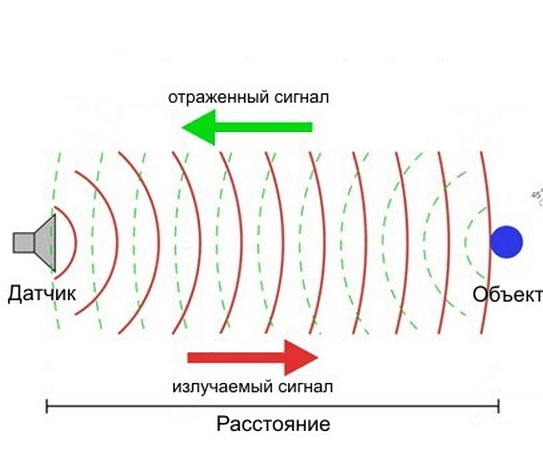
\includegraphics[width=0.7\linewidth]{images/screenshot001}
	\caption{Принцип работы ультразвукового дальномера}
	\label{fig:screenshot001}
\end{figure}

Расстояние до объекта \(L\) можно определить по скорости ультразвуковых волн:
\[s=\frac{vt}{2},\]
где \(v\) - скорость звука, которая отличается для различных сред. Она зависит в основном от плотности среды, в которой звук распространяется. Для воздуха при обычной температуре и плотности скорость звука составляет \(v=343 \text{ м/с}\);\\
\(t\) - время пролета ультразвуковой волны

\subsection{Источник ультразвука}
В воздушной среде используются частоты 30–100 кГц. В излучателях этих колебаний применяются электростатические, пьезоэлектрические, а так же магнитострикционные преобразователи электрического сигнала в ультразвук. Приемники устроены по принципу обратимых электроакустических преобразователей такого же принципа действия. Наибольшее распространение в приемниках и передатчиках получил прямой и обратный пьезоэффекты. Один и тот же обратимый преобразователь может использоваться и на излучение и на прием путем циклического переключения режима работы.

Возбуждение и прием УЗ-волн в используемом датчике осуществляется пьезоэлектрическим способом. Пьезоэлектрический материал обладает свойством, что под действием приложенного к нему механического воздействия на его поверхности возникают электрические заряды. Это называет прямой пьезоэлектрический эффект. Обратный ему происходит в случае, когда на приложенной электрическое напряжение материал реагирует изменением своей формы. Прямой эффект используется для измерений, обратный для генерации УЗ-волн. На рис.~\ref{fig:screenshot002}А показана типовая схема ультразвукового преобразователя, а на рис.~\ref{fig:screenshot002}Б его внешний вид и устройство

\begin{figure}[H]
	\centering
	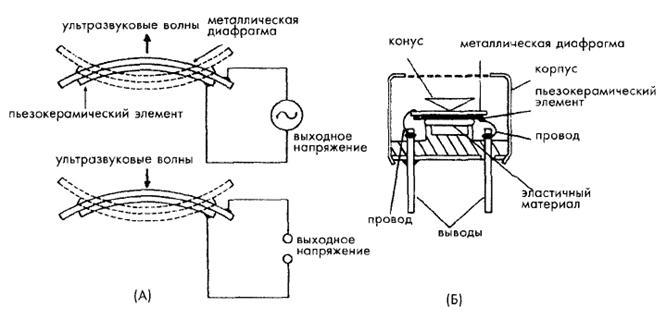
\includegraphics[width=0.7\linewidth]{images/screenshot002}
	\caption{Устройство пьезоэлектрического преобразователя}
	\label{fig:screenshot002}
\end{figure}

\subsection{Влияние расположения объекта и типа поверхностей на результат измерения дальности}
Часто на практике важно знать \textbf{диаграмму направленности датчика}. На рис.~\ref{fig:screenshot003} представлена диаграмма направленности типичного ультразвукового дальномера. \textbf{Диаграмма направленности} - это зависимость распределения интенсивности ультразвукового пучка от угла расхождения по отношению к центральной (акустической) оси, представленная в полярных координатах.

\begin{figure}[H]
	\centering
	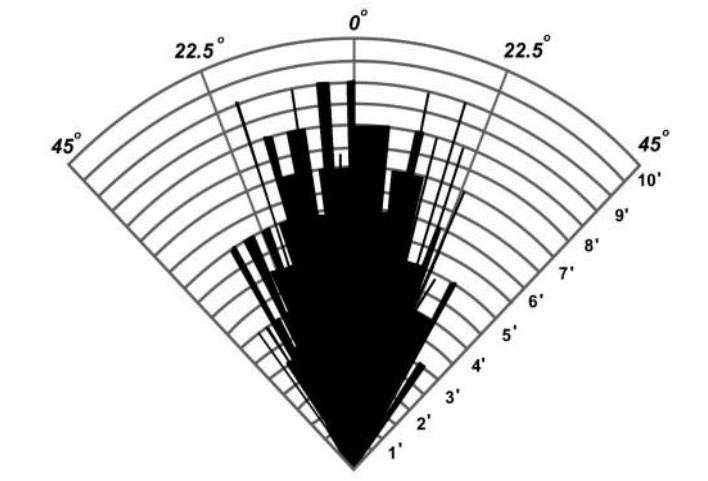
\includegraphics[width=0.4\linewidth]{images/screenshot003}
	\caption{Диаграмма направленности УЗ преобразователя (см. \url{http://www.superrobotica.com/S320110.htm})}
	\label{fig:screenshot003}
\end{figure}

На диаграмме видно, что угол обзора типичного УЗ дальномера составляет примерно 30-45 градусов. Для распространенного варианта использования, когда датчик детектирует препятствия перед собой, такой угол обзора вполне пригоден. Т.е., если объект, даже имеющий малые размеры (но много больше длины УЗ волны), находиться в зоне обнаружения, то он будет определен. 

\begin{figure}[H]
	\centering
	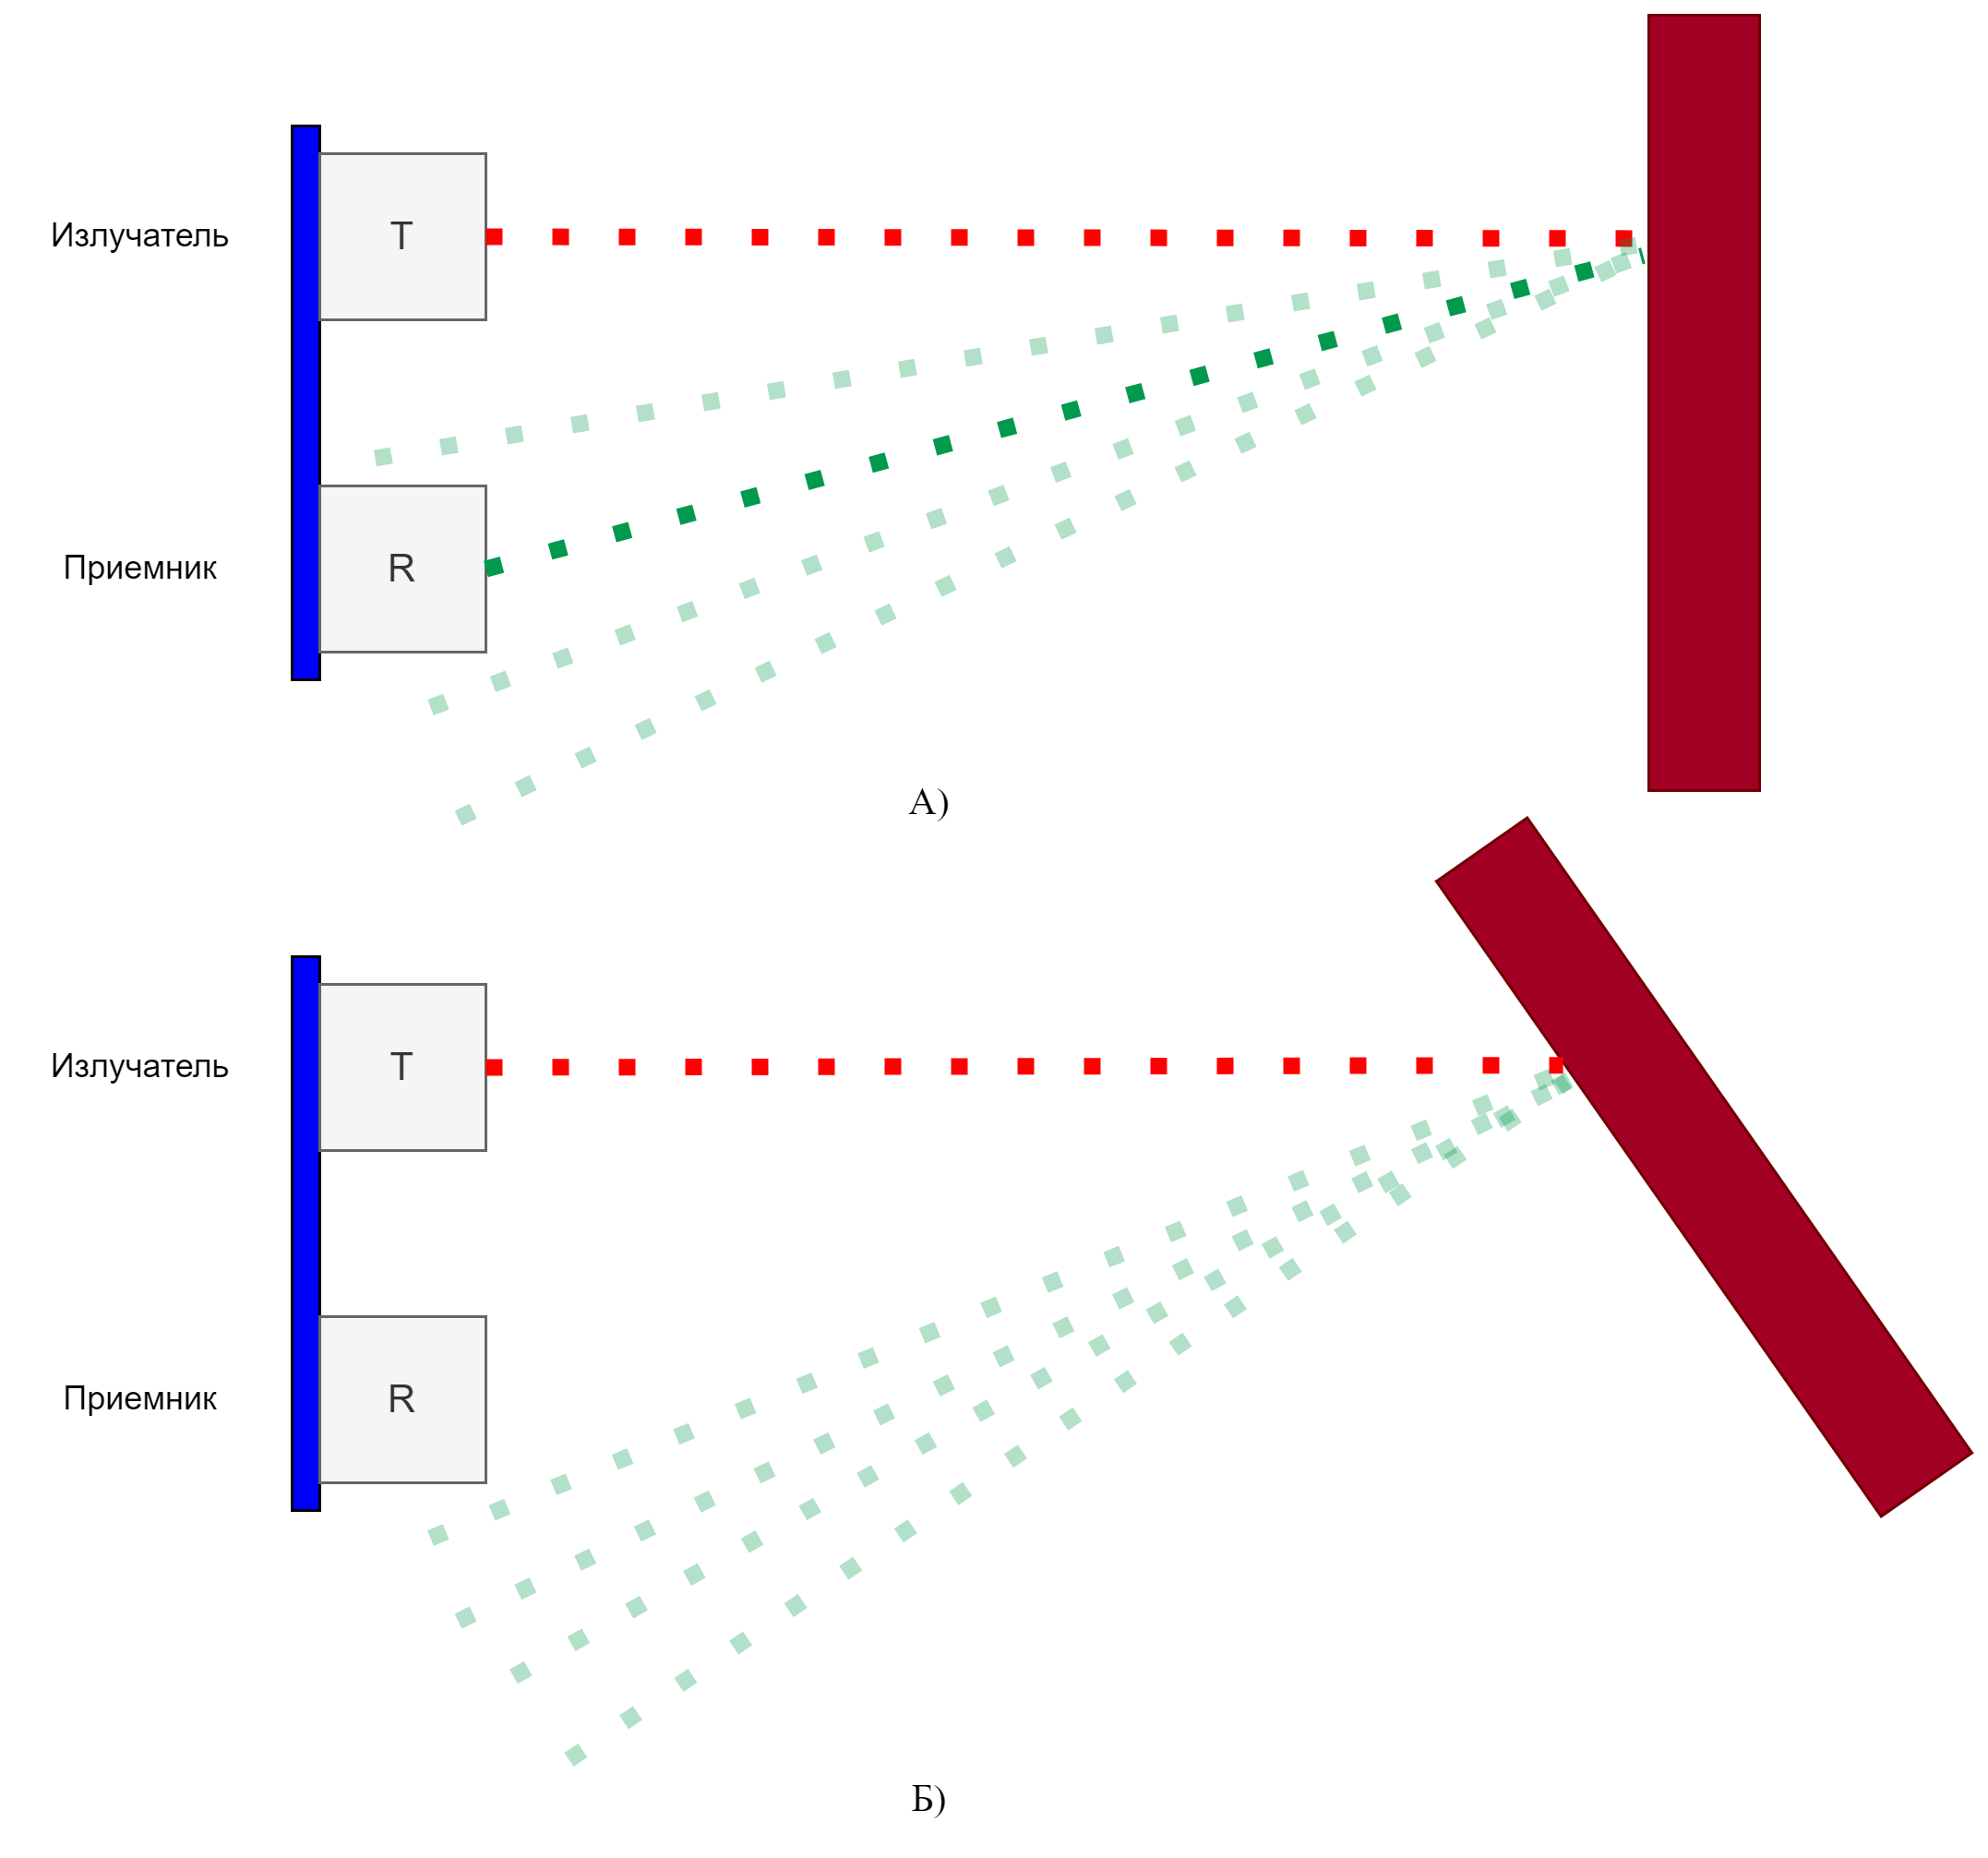
\includegraphics[width=0.65\linewidth]{images/us_ortogonal}
	\caption{Отражение УЗ от плоскости объекта: А) - от перпендикулярной плоскости; Б) - от плоскости под углом}
	\label{fig:us_ortogonal}
\end{figure}

Идеальный случай, когда плоскость объекта расположена перпендикулярно УЗ датчику (рис.~\ref{fig:us_ortogonal}А). Тогда гарантировано отраженная волна попадет в приемник. Однако, если плоскость объекта расположена под таким критическим углом (рис.~\ref{fig:us_ortogonal}Б), что ни одна отраженная волна не попадают на приемник, то обнаружение невозможно. В таком случае измерения будут неадекватные и содержать ошибку.

Искажать измерения УЗ дальномера могут поверхности, хорошо поглощающие звуковые волны. К таким относятся поверхности,имеющие пористую структуру. Измерения дальности до таких поверхностей могу вызывать проблемы.

\subsection{Ультразвуковой дальномер HC-SR04}

Широкое распространение получил УЗ дальномер HC-SR04. Он состоит из двух УЗ преобразователей - передатчик (Transmitter) и приемник (Receiver), установленных на плату с управляющей электроникой. В табл.~\ref{table:techspec} приведены его технические характеристики.

\begin{table}[H]
	\centering
	\caption{Характеристики HC-SR04}\label{table:techspec}
	\begin{tabular}{c|c}
		\toprule
		Напряжение питания & 5 В \\
		\hline
		Потребляемый ток & 	2 мА в режиме ожидания,
							15 мА в режиме передачи\\
		\hline
		Рабочая частота ультразвука & 40 кГц \\
		\hline
		Измеряемая дальность & 2 - 400 см \\
		\hline
		Точность & 0,3 мм \\
		\hline
		Угол обзора & \(15^{\circ}\)\\
		\hline
		Рабочая температура & -30 ... 80 \(^{\circ}\)C  \\
		\hline
		\bottomrule
	\end{tabular}
\end{table}


Принцип работы датчика HC-SR04 изображен на рис.~\ref{fig:screenshot004}.

\begin{figure}[H]
	\centering
	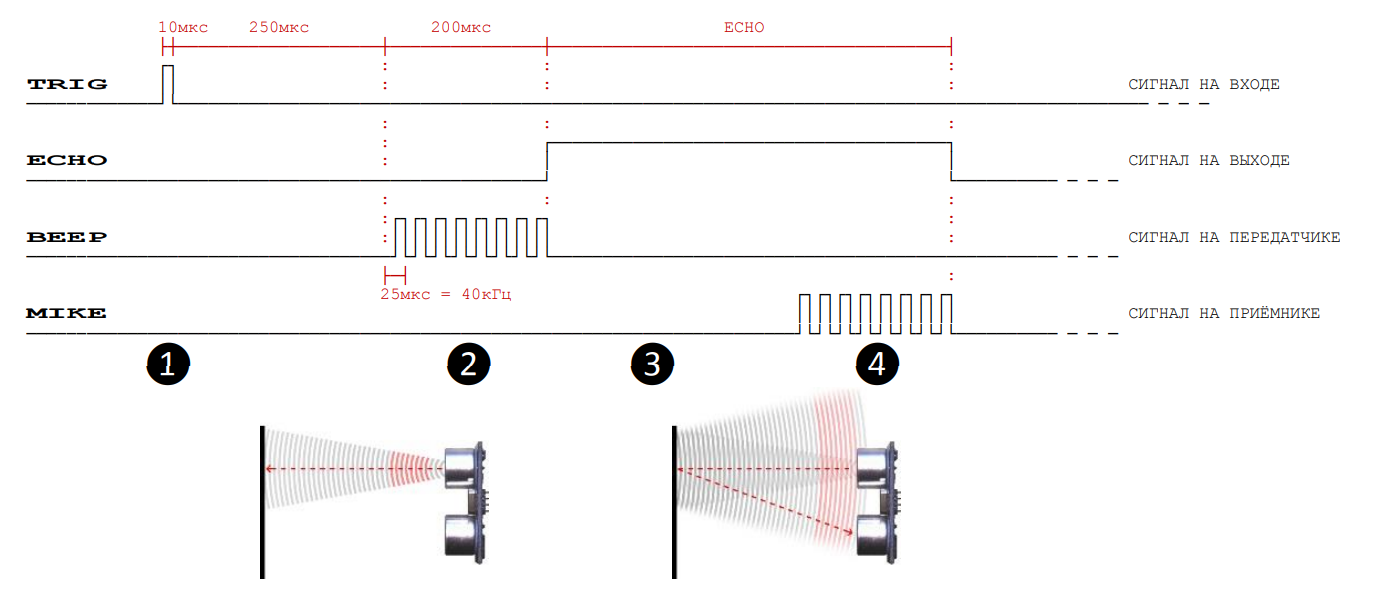
\includegraphics[width=1.0\linewidth]{images/screenshot004}
	\caption{Схема работы датчик HC-SR04}
	\label{fig:screenshot004}
\end{figure}

На рис.~\ref{fig:screenshot005} приведен изображение внешнего вида датчика. Выводы расположены снизу с шагом 2,54 мм. В табл.~\ref{table:pinout} приведено описание выводов датчика.

\begin{figure}[H]
	\centering
	\begin{minipage}[b]{0.45\textwidth}
		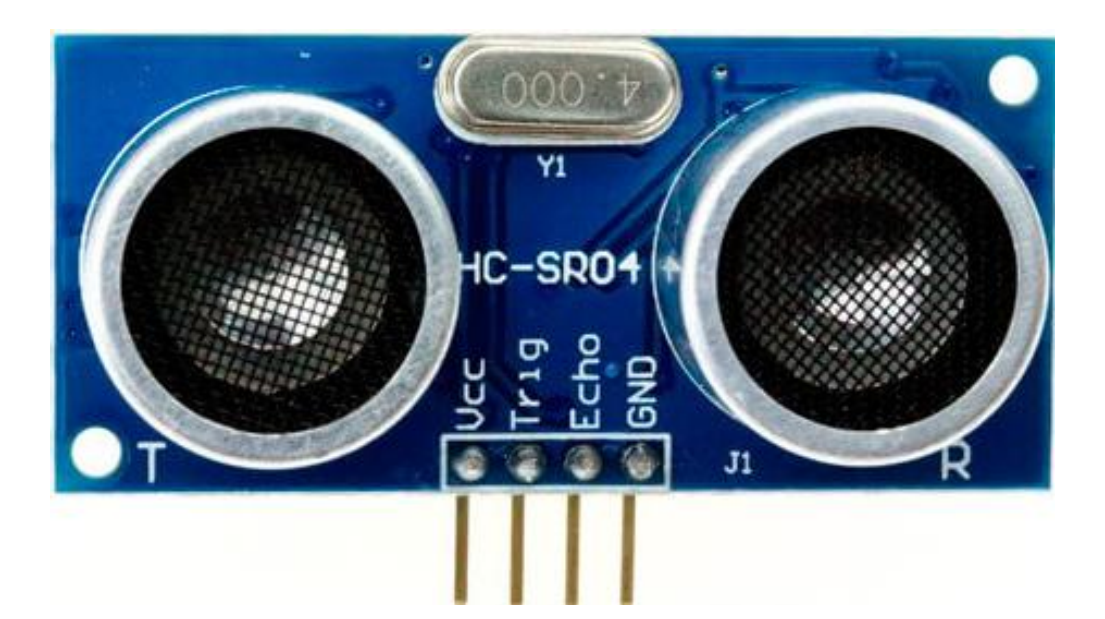
\includegraphics[width=\textwidth]{images/screenshot005}
		\caption{Внешний вид и распиновка HC-SR04}
		\label{fig:screenshot005}
	\end{minipage}
	\hfill
	\begin{minipage}[b]{0.45\textwidth}
		\begin{table}[H]
			\centering
			\caption{Характеристики HC-SR04}\label{table:pinout}
			\begin{tabular}{c|c|c}
				\toprule
				VCC & Питание & V+ \\
				\hline
				TRIG & Вход & Стартовый импульс\\
				\hline
				ECHO & Выход & Сигнал ожидания \\
				\hline
				GND & Питание & V- (общий) \\
				\bottomrule
			\end{tabular}
		\end{table}
	\end{minipage}
\end{figure}

\newpage
\textbf{Цикл измерения дальности делится на 4 этапа:}
\begin{enumerate}
	\item Вывод датчика из режима ожидания. Требуется подать стартовый импульс на вход TRIG (положительный импульс длительностью 10 мкс).
	\item Датчик генерирует меандр длиной  8 импульсов с периодом 25 мкс (что соответствует частоте 40кГц) на ультразвуковой передатчик (Transmitter).
	\item По спаду последнего сгенерированного импульса, датчик устанавливает уровень логической «1» на выходе ECHO. Одновременно с этим, датчик ждет получение отраженной ультразвуковой волны той же частоты на ультразвуковой приемник (Receiver). \hl{\textbf{То есть, длительность импульса на выводе ECHO пропорциональна расстоянию до объекта}}.
	\item После получения последнего импульса отраженной волны, датчик переходит в режим ожидания, устанавливая уровень логического «0» на выходе ECHO. Аналогичные действия будут совершены, если в течении 38 мс датчик не примет отраженную ультразвуковую волну (тайм-аут). В результате время наличия логической «1» на выходе ECHO равно времени прохождения ультразвуковой волны от датчика до препятствия и обратно.
\end{enumerate}

\subsection{Расчет расстояния до объекта}
Расстояние до объекта \(L\) вычисляется умножением скорости на время (в данном случае скорости звуковой волны, на время ожидания эха). Но так звуковая волна проходит расстояние до объекта и обратно, поэтому пройденное расстояние следует разделить на 2:
\begin{equation}
	L = \frac{1}{2} v \tau,
	\label{eq:1}
\end{equation}
где \(L\) - вычисленное расстояние УЗ-датчиком, м; \\
\(v\) - скорость звука в воздухе, м/с; \\
\(\tau\) - время ожидания эха (длительность импульса с выхода ECHO датчика), с.

Однако, скорость звука в воздухе величина не постоянная и зависит от температуры, т.е.:
\begin{equation}
	v^2 = \gamma \frac{RT}{M},
	\label{eq:2}
\end{equation}
где \(\gamma=\frac{7}{5}\) - показатель адиабаты воздуха; \\
\(R=8,31 \text{ Дж/моль \(\cdot\) К}\) - универсальная газовая постоянная; \\
\(T = t^\circ C + 273,15 K\) - абсолютная температура воздуха; \\
\(M = 0,02898 \text{кг/моль}\) - молекулярная масса воздуха.

Время ожидания пролета УЗ волны до объекта и обратно \(\tau\) можно получить от датчика, измерив длительность импульса на выводе ECHO. Длительность импульса ECHO \(\tau_{echo}\) следует измерять в микросекундах для достижения высокой точности. 

Подставив в уравнение~\ref{eq:2} известные константы \(\gamma\), \(R\), \(M\), и объединив с формулой~\ref{eq:1} получим формулу для расчета расстояния в миллиметрах:
\begin{equation}
	v = 20.042 \sqrt{t+273.15}, \\
\end{equation}
\begin{equation}
	L \approx \tau_{echo} \frac{\sqrt{t+273.15}}{100},
\end{equation}
где \(v\) - скорость УЗ волны с учетом констант и абсолютной температуры, м/с; \\
\(L\) - расстояние до объекта, мм; \\
\(\tau_{echo}\) - длительность импульса ECHO, мкс; \\
\(t\) - температура воздуха, \(^\circ C\).


\section{Ход работы}
\subsection{Подключение}
Подключите модуль ``Микроконтроллер ATMEGA32'', модуль ``Модуль датчиков'' к внешнему блоку питания (или у портам USB компьютера/ноутбука) с помощью кабеля USB. Выполните коммутацию модулей приборными проводами в соответствии с таблицей~\ref{labtable}  и с рис.~\ref{labscheme}. К контроллеру необходимо подсоединить датчики расстояния - Инфракрасный и Ультразвуковой.

\begin{figure}[H]
	\centering
	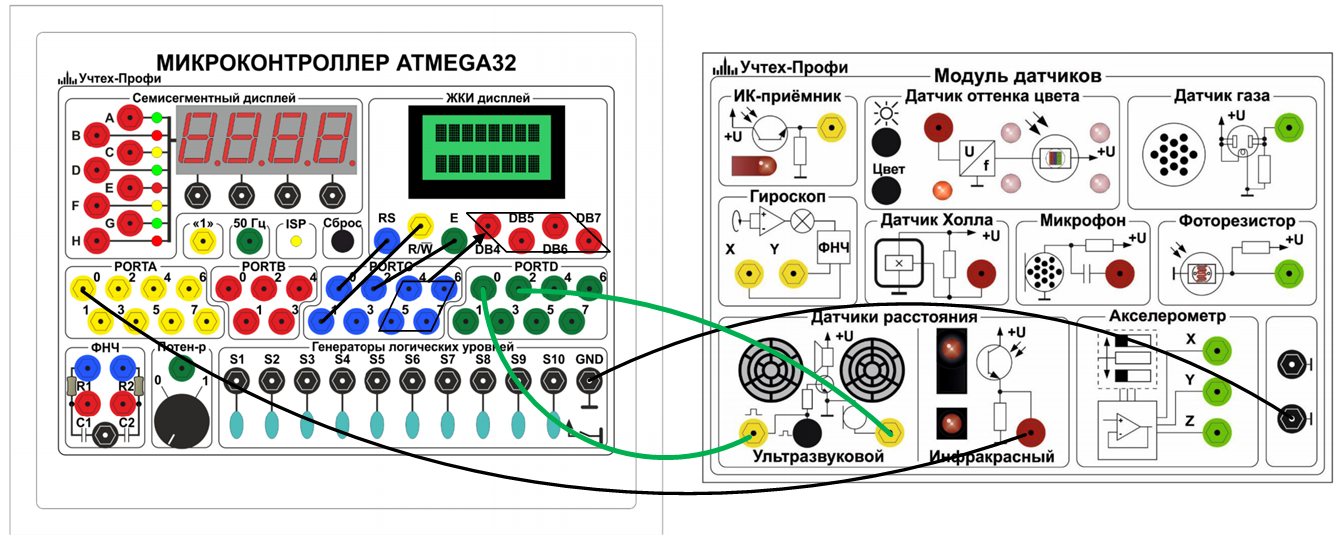
\includegraphics[scale=0.65]{images/lab4-scheme.png}
	\caption{Схема подключения модулей}\label{labscheme}
\end{figure}
\begin{table}[H]
	\caption{Коммутация модулей}\label{labtable}
	\begin{longtable}[]{@{}l|l@{}}
		\toprule
		Порт микроконтроллера ATMEGA32 & Назначение \\
		\midrule
		\endhead
		PORTC:0 & ЖК-дисплей: RS \\
		PORTC:1 & ЖК-дисплей: R/W \\
		PORTC:2 & ЖК-дисплей: E \\
		PORTC:4-7 & ЖК-дисплей: DB4-DB7 \\
		PORTA:0 & Инфракрасный дальномер \\
		PORTD:0 & Ультразвуковой дальномер TRIG \\
		PORTD:2 & Ультразвуковой дальномер ECHO \\
		\bottomrule
	\end{longtable}  
\end{table}

\subsection{Использование кода}

Для проведения измерений в лабораторной работе необходимо загрузить программу в микроконтроллер ATMEGA32. Скачайте код из репозитория GitHub \url{https://github.com/albatron22/Lab_sens-4} В папке \texttt{/src} лежат файлы исходного кода программы. Заголовочные файлы подключаемых модулей находятся \texttt{/include}. Основной выполняемый код находится в файле \texttt{/src/main.cpp}. Откройте его и проанализируйте код, который в нём содержится.

\textbf{Порядок загрузки программы в модуль ``Микроконтроллер ATMEGA32''}
\begin{enumerate}
	\item Подключите модуль к компьютеру или ноутбуку через USB провод.
	\item В диспетчере устройств проверьте номер COM-порта, который был присвоен модулю. Обновите номер порта \texttt{UPLOAD\_PORT} в файле \texttt{platformio.ini}.
	
	\item Запустите компиляцию и сборку прошивки нажав на кнопку ``Build'' на нижней панели VSCode. Затем загрузите файл прошивки в память микроконтроллера нажав на кнопку ``Upload''.
\end{enumerate}
 

После этого на ЖК-дисплее отобразятся измеренные расстояния с обоих датчиков. В \textbf{верхней строк}е расстояние с ИК-дальномера \(L_{IR}\), в \textbf{нижней строке} УЗ-дальномера \(L_{US\\}\).

\subsection{Проведение измерений}

Необходимо получить \(N=20\) измерений расстояний \(L_{IR}\) и \(L_{US}\) при различном расстоянии от датчика до плоского предмета в пределах диапазона 10-80 см (здесь мы вынуждены ограничится рабочим диапазоном ИК-дальномера, который меньше диапазона УЗ-дальномера). Используйте рулетку или линейку для измерения истинного расстояния.

В Лабораторной работе № 3 вами были получены параметры \(k\) и \(b\) характеристики ИК-дальномера. Их необходимо ввести в программный код для расчета расстояния.

\begin{verbatim}
	/* Параметры характеристики ИК-дальномера, найденные в Лабораторной работе № 3 */
	/* ИСПОЛЬЗУЙТЕ СВОИ ЗНАЧЕНИЯ */
	const float ir_k = 0.0f; // k
	const float ir_b = 0.0f; // b
\end{verbatim}

Код для работы с УЗ-дальномером \textbf{требуется написать самостоятельно} по алгоритму на рис.~\ref{fig:algoritm}.

\begin{figure}[H]
	\centering
	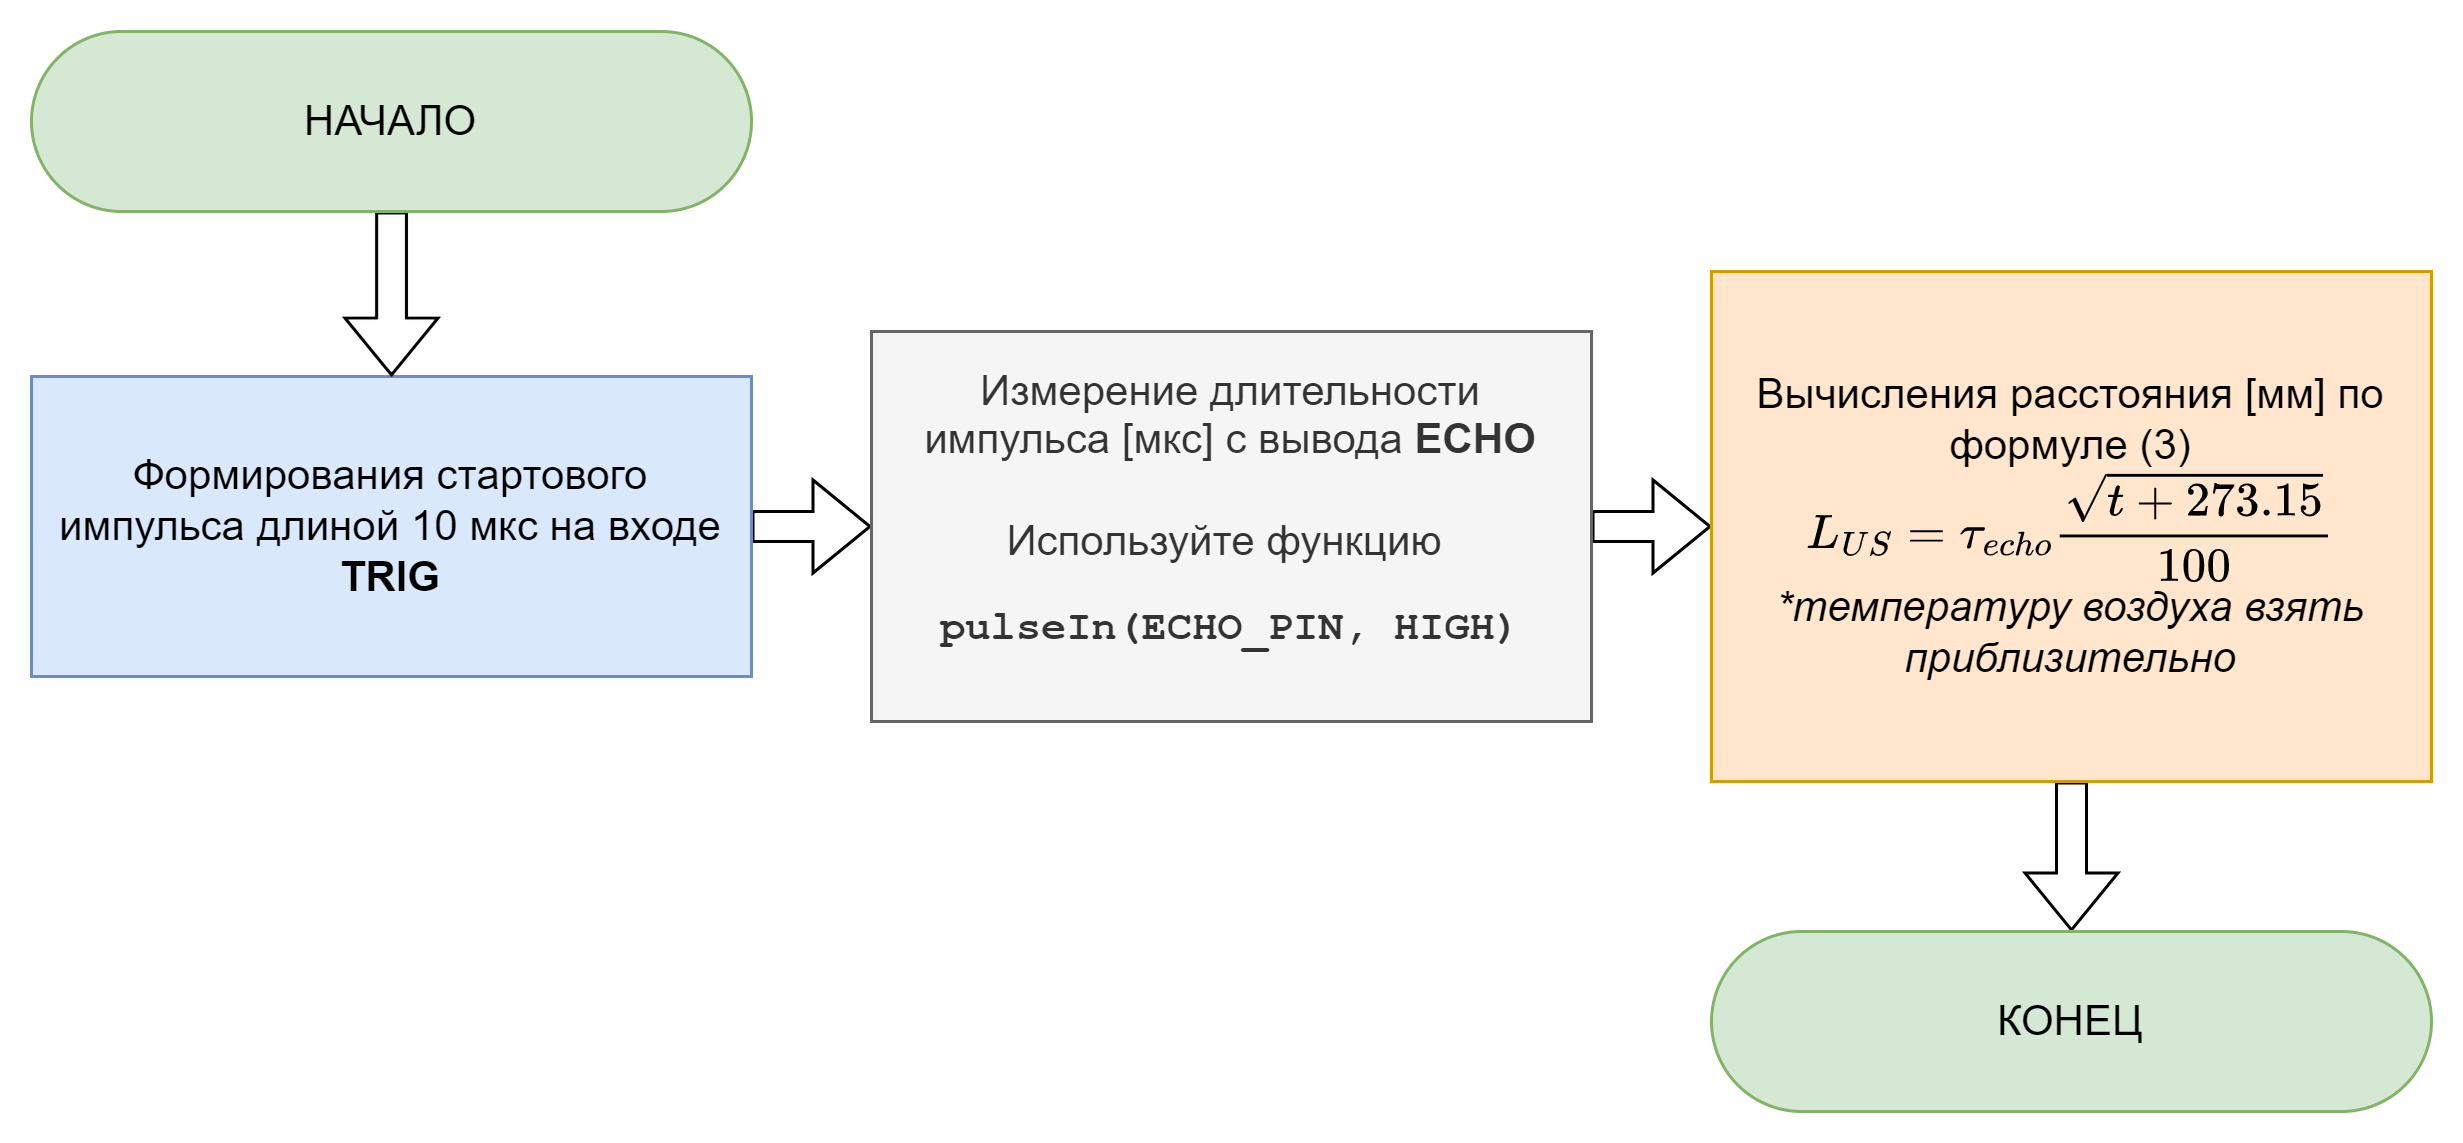
\includegraphics[width=1.0\linewidth]{images/algoritm}
	\caption{Блок-схема алгоритма работы с УЗ-дальномеров}
	\label{fig:algoritm}
\end{figure}

Заполните таблицу~\ref{exper} (только первые три колонки), где каждому реальному расстоянию \(L(i)\) в мм (по линейке/рулетке) соответствует расстояния с ИК-дальномера \(L_{IR}(i)\) и УЗ-дальномера \(L_{US}(i)\), \(i=\overline{1,\:20}\) 

\begin{table}[H]
	\centering
	\caption{Результаты}\label{exper}
	\begin{longtable}{c|c|c|c|c|c|c|c}
		\toprule
		№ измерения \(i\) & \(L\), мм & \(L_{IR}\), мм & \(L_{US}\), мм  & \(\Delta_{IR}\), мм & \(\delta_{IR}\), \% & \(\Delta_{US}\), мм & \(\delta_{US}\), \% \\
		\midrule
		1 &&&&&&& \\
		\hline
		2 &&&&&&& \\
		\hline
		3 &&&&&&& \\
		\hline
		\dots &&&&&&& \\
		\hline
		20 &&&&&&& \\
		\bottomrule
	\end{longtable}
\end{table}

\subsection{Обработка измерений}

\begin{enumerate}
	
	\item Вычислить и занести в таблицу~\ref{exper}. абсолютные погрешности измерения расстояния \(\Delta_{IR}\) и \(\Delta_{US}\) для ИК и УЗ дальномеров соответственно по формулам:
	\[\Delta_{IR} = |L - L_{IR}|,\]
	\[\Delta_{US} = |L - L_{US}|.\]
	
	\item Определить и занести в таблицу~\ref{exper} относительные погрешности \(\delta_{IR}\) и \(\delta_{US}\) для ИК и УЗ дальномеров соответственно по формулам:
	\[\delta_{IR} = \frac{\Delta_{IR}}{L_{IR}} \cdot 100\%,\]
	\[\delta_{US} = \frac{\Delta_{US}}{L_{US}} \cdot 100\%.\]
	
	\item Построить следующие 2 графика:
	\begin{itemize}
		\item совмещенный график зависимостей \textbf{абсолютной ошибки} дальномеров от фактического расстояния \(\Delta_{IR}(L)\) и \(\Delta_{US}(L)\).
		
		\item совмещенный график зависимостей \textbf{относительной ошибки} дальномеров от фактического расстояния \(\delta_{IR}(L)\) и \(\delta_{US}(L)\).
	\end{itemize}
	
	\item Сформулируйте вывод о сравнительной точности работы двух типов датчиков.
\end{enumerate}

\section{Вопросы}

\begin{enumerate}
	\item Принцип действия и область применения УЗ-дальномера.
	\item Источник ультразвука. Влияние внешних условия на качество измерений расстояния УЗ-дальномером.
	\item Устройство и характеристики типового УЗ-дальномера (на примере HC-SR04). Цикл работы датчика.
	\item Алгоритм расчет расстояния до объекта на основе выхода УЗ датчика (показать код расчета расстояния и прокомментировать его).
	\item Сравнительные преимущества и недостатки оптического (ИК) и акустического (УЗ) типов дальномеров.
\end{enumerate}


\end{document}